 Além disso, o reprodutor de mídia recebe comandos de apresentação, controla todas as máquinas de estado de evento e responde a consultas do formatador (Ginga-NCL). Para favorecer a incorporação de media players de terceiros em um motor de apresentação NCL, sugere-se um projeto modular, com o objetivo de separar os media players do motor de apresentação (NCL player). A Figura~\ref{fig:mediaPlayer} ilustra uma organização modular para um ambiente de apresentação NCL. Para usar um terceiros com interfaces que não são compatíveis com o exigido pelo mecanismo de apresentação, é necessário desenvolver módulos, chamados adaptadores, para fazer as adaptações necessárias. Nesse caso, o media player consiste em um adaptador junto com o próprio player \cite{ITU:2009ma}.

\begin{figure}[!h]
    \centering
    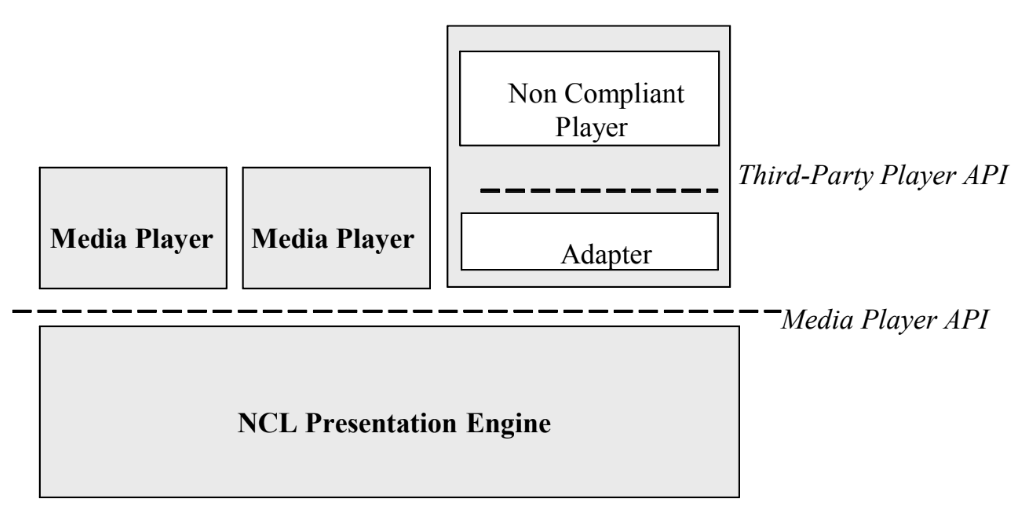
\includegraphics  [scale=0.4,keepaspectratio=true]{figuras/IntegracaoMediaPlayer.png}
    \caption{APIs para integração de reprodutores de mídia com uma implementação de mecanismo de apresentação NCL \cite{ITU:2009ma}}
    \label{fig:mediaPlayer}
\end{figure}

Os reprodutores de mídia devem controlar a máquina de estado de evento daquela mídia e relatar qualquer alteração nessa máquina ao reprodutor NCL. Portanto, além de definir uma interface para receber comandos vindos do reprodutor NCL, a API do reprodutor de mídia deve também definir uma interface para relatar mudanças de estado de evento da máquina para o reprodutor NCL. Para colocar um objeto de mídia em execução, o reprodutor NCL deve primeiro instanciar o reprodutor de mídia apropriado (pode haver mais de uma instância de um mesmo reprodutor de mídia), que deve seguir a especificação da API definida na Tabela\ref{tab:mediaAPI} para se comunicar com o player NCL.

\begin{table}[h]
\label{tab:mediaAPI}
\caption{Media player API}
\centering
{
  % distancia entre a linha e o texto
  \renewcommand\arraystretch{1.25}
  \begin{tabular}{|p{5cm}|p{10cm}|} \hline
   \multicolumn{1}{|c|}{Implementado pelo:} & \multicolumn{1}{c|}{Operação (parâmetros de entrada)}  \\\hline 
   Media player & prepare (mediaType media) \\\hline
   Host NCL player & notifyAudioBuffer (any buffer) \\\hline
   Host NCL player & notifyVideoBuffer (any buffer)\\\hline
   Media player & setPropertyValue(string name, string value, string duration, string by) \\\hline
   Media player & requestPropertyValue(string name) \\\hline
   Host NCL player & notifyPropertyValue (string name, string value)\\\hline
   Media player & setAction (ID eventId, actionType action) \\\hline
   Host NCL player & notifyEventTransition (ID eventId, transitionType transition) \\\hline
   Media player & addEvent (eventType event) \\\hline
   Media player & removeEvent (ID eventId) \\\hline
   Host NCL player & notifyError(string message) \\\hline
  \end{tabular}
}
\end{table}

A operação prepare, disparada pelo reprodutor NCL, informa ao reprodutor de mídia os seguintes parâmetros: as propriedades associadas ao objeto de mídia para o qual o reprodutor de mídia foi criado, a lista de eventos (apresentação, seleção, atribuição, etc.) que precisam ser monitorados pelo reprodutor de mídia e a localização do conteúdo de mídia a ser executado/apresentado.

Se o conteúdo não puder ser localizado ou se o reprodutor de mídia não souber como lidar com o tipo de conteúdo, o reprodutor de mídia finaliza a operação de preparação sem realizar nenhuma ação e relatar uma mensagem de erro (\textit{notifyError(string message)}). Se a operação for bem-sucedida, as áreas de memória a serem preenchidas pelo reprodutor de mídia são identificadas e retornadas, dependendo do tipo de mídia a ser apresentada, por meio das operações \textit{notifyAudioBuffer} e \textit{notifyVideoBuffer}.

A interface \textit{setPropertyValue} permite ao formatador NCL definir valores para as propriedades do objeto de mídia em execução controlada pelo reprodutor de mídia. Por exemplo, usando o \textit{setPropertyValue}, o formatador pode passar um parâmetro de entrada usado pelo reprodutor de mídia ao executar a apresentação. 

A interface requestPropertyValue permite que o formatador obtenha valores de propriedade do objeto de mídia em execução controlada pelo reprodutor de mídia. O valor é retornado quando o reprodutor de mídia notifica o formatador por meio da interface \textit{notificationPropertyValue}. O formatador NCL pode enviar ações (iniciar (start), parar(stop), etc.) para alterar o estado de um evento (disparar transições na máquina de estado do evento controlada pelo reprodutor de mídia) por meio da interface setAction. Os reprodutores de mídia devem notificar o formatador sobre as alterações nas máquinas de estado do evento que ele controla. As alterações de estado do evento são notificadas por meio da interface \textit{notificationEventTransition}. Os eventos podem ser adicionados ou removidos da lista de eventos usando as operações \textit{addEvent} e \textit{removeEvent}, respectivamente.





\begin{table}[h]
\label{tab:modulosNCl}
\caption{Área Funcionais da Linguagem NCL 3.0 \cite{soares2009programando}}
\centering
{
  % distancia entre a linha e o texto
  \renewcommand\arraystretch{1.0}
  \begin{tabular}{|p{4.5cm}|p{6cm}|p{4cm}|} \hline
   \multicolumn{1}{|c|}{Áreas Funcionais} & \multicolumn{1}{c|}{Módulos} & \multicolumn{1}{c|}{Elementos} \\\hline 
   
   \multirow{3}{*}{Structure} & \multirow{3}{*}{Structure} & ncl\\\cline{3-3} && head\\\cline{3-3} && body\\\hline
   
   \multirow{2}{*}{Layout} & \multirow{2}{*}{Layout} & regionBase\\\cline{3-3} && region\\\hline
   \multirow{2}{*}{Components} & Media & media\\\cline{2-3} & Context & context\\\hline
   
   \multirow{4}{*}{Interfaces} & MediaContentAnchor & area\\\cline{2-3}
   & PropertyAnchor & property\\\cline{2-3}
   & CompositeNodeInterface & port\\\cline{2-3}
   &\multirow{2}{*}{SwitchInterface} & switchPort\\\cline{3-3} && mapping \\\hline
   
   \multirow{3}{*}{Presentation Specification} & \multirow{3}{*}{Descriptor} & descriptor \\\cline{3-3} 
   && descriptorParam \\\cline{3-3} && descriptorBase \\\hline
   
   \multirow{4}{*}{Linking} & \multirow{4}{*}{Linking} & bind\\\cline{3-3} && bindParam\\\cline{3-3} && linkParam\\\cline {3-3} && link\\\hline
      
   \multirow{11}{*}{Connectors} & \multirow{10}{*}{CausalConnectorFunctionality} & causalConnector\\\cline{3-3}&&
   connectorParam\\\cline{3-3} && simpleCondition\\\cline {3-3} && compoundCondition\\\cline{3-3} && simpleAction\\\cline{3-3} &&
   compoundAction\\\cline{3-3} && assessmentStatement\\\cline{3-3} &&
   attributeAssessment\\\cline{3-3} && valueAssessment\\\cline{3-3} &&
   compoundStatement\\\cline{2-3} & ConnectorBase & connectorBase \\\hline
  
  \multirow{8}{*}{Presentation Control} & \multirow{3}{*}{TestRule} & ruleBase\\\cline{3-3}
  && rule\\\cline{3-3} && compositeRule\\\cline{2-3} &
  TestRuleUse & bindRule\\\cline{2-3} &
  \multirow{2}{*}{ContentControl} & switch\\\cline{3-3} &&
  defaultComponent\\\cline{2-3} &
  \multirow{2}{*}{DescriptorControl} & descriptorSwitch\\\cline{3-3} &&
  defaultDescriptor\\\hline
  
  Timing &  Timing & \\\hline
  
  \multirow{5}{*}{Reuse} & \multirow{3}{*}{Import} & importBase\\\cline{3-3}
  && importDocumentBase\\\cline{3-3} && importNCL\\\cline{2-3} &
  EntityReuse &\\\cline{2-3} & ExtendedEntityReuse &\\\hline
  
  Navigational Key &  KeyNavigation & \\\hline 
  
  Animation &  Animation & \\\hline 
 
   \multirow{2}{*}{Transition Effects} & TransitionBase & transitionBase\\\cline{2-3}
  & Transition & transition\\\hline
  
  EntityReuse &\\\cline{2-3} & ExtendedEntityReuse &\\\hline
   EntityReuse &\\\cline{2-3} & ExtendedEntityReuse &\\\hline
   EntityReuse &\\\cline{2-3} & ExtendedEntityReuse &\\\hline
 
  \end{tabular}
}
\end{table}